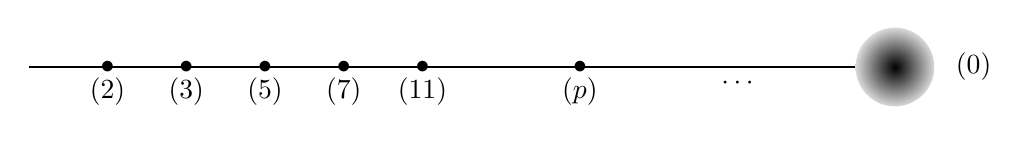
\begin{tikzpicture}
% Non-zero primes (closed points)
\draw[thick] (0,0)
    -- (1,0) node {\(\bullet\)} node[below] {\((2)\)}
    -- (2,0) node {\(\bullet\)} node[below] {\((3)\)}
    -- (3,0) node {\(\bullet\)} node[below] {\((5)\)}
    -- (4,0) node {\(\bullet\)} node[below] {\((7)\)}
    -- (5,0) node {\(\bullet\)} node[below] {\((11)\)}
    -- (7,0) node {\(\bullet\)} node[below] {\((p)\)}
    -- (9,0) node[below] {\(\cdots\)}
    -- (11,0);
% Generic point
\shade[inner color=black, outer color=gray!30]
    (11,0) circle (0.5);
\draw (12,0) node {\((0)\)};
\end{tikzpicture}